%SAVEDAT= 1453457093
\documentclass[11pt, a4paper]{article} 
\usepackage{slashed,jheppub,multirow,relsize,soul}
\usepackage[normalem]{ulem}


\newcommand{\refeq}[1]{Eq.~(\ref{#1})}
\newcommand{\refeqs}[2]{Eqs.~(\ref{#1})~and~(\ref{#2})}
\newcommand{\refeqss}[3]{Eqs.~(\ref{#1}), (\ref{#2})~and~(\ref{#3})}
\newcommand{\reffig}[1]{Fig.~\ref{#1}}
\newcommand{\reffigs}[2]{Figs.~\ref{#1}~and~\ref{#2}}
\newcommand{\refsec}[1]{Section~\ref{#1}}
\newcommand{\refapp}[1]{Appendix~\ref{#1}}
\newcommand{\reftab}[1]{Table~\ref{#1}}
\newcommand{\refref}[1]{Ref.~\cite{#1}}
\newcommand{\refrefs}[2]{Refs.~\cite{#1}~and~\cite{#2}}

\def\abelian{abelian}
\def\nonabelian{non-abelian}
\def\lagrangian{lagrangian}
\def\eg{\emph{e.g.}}
\def\ie{\emph{i.e.}}
\def\aka{\emph{a.k.a.}}
\def\muboone{MicroBooNE}
\def\minerva{MINER$\nu$A}

%%%%%%% A few editorial macros. %%%%%%%

\newcommand{\lorem}{ \textcolor[rgb]{0.8,0.8,0.8}{Lorem ipsum dolor sit amet, consectetur
adipiscing elit, sed do eiusmod tempor incididunt ut labore et dolore magna
aliqua. Ut enim ad minim veniam, quis nostrud exercitation ullamco laboris nisi
ut aliquip ex ea commodo consequat. Duis aute irure dolor in reprehenderit in
voluptate velit esse cillum dolore eu fugiat nulla pariatur. Excepteur sint
occaecat cupidatat non proident, sunt in culpa qui officia deserunt mollit anim
id est laborum.}}

\newcounter{CommentCount}
\setcounter{CommentCount}{1}

\newcommand{\marcom}[2]{\textsuperscript{\textcolor{#1}{\theCommentCount}}\marginpar{\textsuperscript{\textcolor{#1}{\theCommentCount}}\textcolor{#1}{{\small#1: #2}}}\stepcounter{CommentCount}}

\newcommand{\newtext}[2]{\textcolor{#1}{\ul{#2}}}

% Add your own colour down here... 
\definecolor{PB}{rgb}{0.9,0,0}
\definecolor{MARK}{rgb}{0.612, 0.153, 0.69}

%%%%%%%%%%%%%%%%%%%%%%%%%%%%%%%%%%%%%%%


\title{MeV mass sterile neutrino decay at short-baseline neutrino facilities}

\author{One}
\author{Two}
\author{Three}

\affiliation{Institute for Particle Physics Phenomenology, Department of
Physics, Durham University, South Road, Durham DH1 3LE, United Kingdom}

\emailAdd{one@durham.ac.uk}
\emailAdd{two@durham.ac.uk}
\emailAdd{three@durham.ac.uk}

\abstract{
%
We study the sensitivity of the Short-Baseline Neutrino (SBN) programme at Fermilab to 
sterile neutrino decay in a variety of models. We show that this experimental complex 
can be expected to extend the known bounds on such decays and comment on the interplay 
between the different beam lines and detector technologies. 
}

\begin{document} 

\maketitle

\section{Introduction}

\lorem\lorem

\section{Short-Baseline Neutrino Complex}

\marcom{PB}{This could also be bundled into the intro...} The Fermilab SBN
programme \cite{Antonello:2015lea} will comprise of a number of detectors in
the Booster Neutrino Beam (BNB): SBND (previously known as LAr1-ND) at 100m
from the target, \muboone\ at 470m and ICARUS-T600 at 600m.

In addition to events arising from the BNB, the detectors of the SBN complex
will also collect events associated with the NuMI beam, currently being used in
the NO$\nu$A, MINER$\nu$A and MINOS+ experiments.

\section{Sterile neutrino decay}

Generically, a gauge-singlet fermion will be unobservable by all
non-gravitational means unless it mixes with the active neutrino sector. The
presence of mixing introduces a range of possible observable signatures
depending on the magnitude of the sterile mass and its mixing to the active
sector. 

The most general renormalizable \lagrangian\ extending the SM to include a
single novel gauge-singlet fermion $N$ is given by
%
\begin{align}   \mathcal{L} = \mathcal{L}_\text{SM} +
\overline{N}i\slashed{\partial}N+ \frac{\mu}{2} \overline{N^\text{c}}N  +
\left( y_\alpha\overline{L}_\alpha\tilde{H} N
+\text{h.c.}\right),\label{eq:minimallag} \end{align}
%
where $y_\alpha$ denote Yukawa couplings and $\mu$ a Majorana mass term for
$N$. The extension to multiple new fermions involves promoting $y$ and $\mu$ to
matrices with indices for the new states, but will offer no real
phenomenological differenes in the current work.\footnote{The minimal single
$N$ extension does not allow for the observed masses of the neutrinos, as the
mass matrix is rank 1. We assume that an appropriate extension has been
performed to statisfy neutrino oscillation data.} Much work has been done
understanding the phenomenology of novel neutral states, which varies
significantly over their large parameter spaces. An important signal for light
sterile neutrinos are possible observable effects in oscillation experiments,
which could alleviate short-baseline oscillation anomalies; although, no
minimal solution seems to provide a particularly compelling improvement
\cite{}. At larger masses, the neutral particles no longer participate in
oscillation, but these models can generate new signatures at beam dump
experiments \cite{}. At even higher masses, these particles could provide a
natural way to suppress the size of active neutrino masses through the Type I
or III see-saw mechanisms \cite{}. 

Generally speaking, once the neutrinos are massive enough to no longer
oscillate but remain light enough to be produced in terrestrial experiments,
the best way to observe them is through their direct decay into SM particles.
In the minimal \lagrangian\ in \refeq{eq:minimallag}, the only direct couplings
to new sterile fermions are neutrino Higgs interactions. However, these
couplings generate off-diagonal neutrino bilinears below the electroweak
symmetry breaking scale, which leads to mixing between the $4+$ flavours of
neutrinos. Such mixing then introduces production and decay mechanisms of many
kinds for the state $N$ through mass insertion on an active neutrino fermion
line. These decays have been studied extensively in the literature
\cite{Atre} and depend only on the size of neutrino mixing to various
flavours, parameterized by the elements of an extended $4\times4$ PMNS matrix,
%
\[ U_{e4}, \qquad U_{\mu 4} \qquad \text{and} \qquad U_{\tau 4},  \]
%
and the mass of the state $N$ itself. The branching ratios for these decays are
shown in \reffig{fig:branchingratios} as a function of mass for two extremes of
the flavour mixing pattern. On the left, we show the branching ratios if the
new state only mixes with all flavours of active neutrino equally
$U_{e4}=U_{\mu 4}=U_{\tau 4}$, and on the right, when the only mixing with with
$\nu_e$ ($U_{\mu 4}=U_{\tau 4} = 0$). The main effect of the flavour structure
is to forbid certain decays which require certain elements. For example, the
decay of a sterile $N$ into a lepton and a charged pion,
%
\[ N \to l^\pm \pi^\mp,   \]
%
only proceeds if $U_{l4}\neq 0$. This, in turn, affects the possible production
mechanisms for these particles. In a conventional neutrino beam, most neutrinos
are derived from meson decay (or secondary $\mu^\pm$ decays). If $U_{e4}=U_{\mu
4}=0$, such decays with a mass insertion for the sterile neutrino are
impossible for pions or kaons. For this reason, we will mainly focus on mixing
with the first two generations. This parameter space will be probed by working
at higher energies, where the neutral fermions can be produced by decays of
charmed mesons such as $D^\pm$, by the SHiPS experiment \cite{}.
 
\begin{figure}[t]
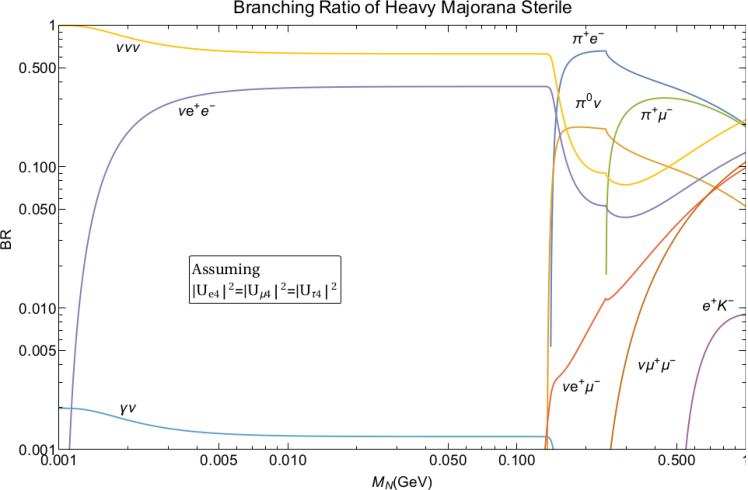
\includegraphics[width=0.49\textwidth]{figures/bounds1.pdf}  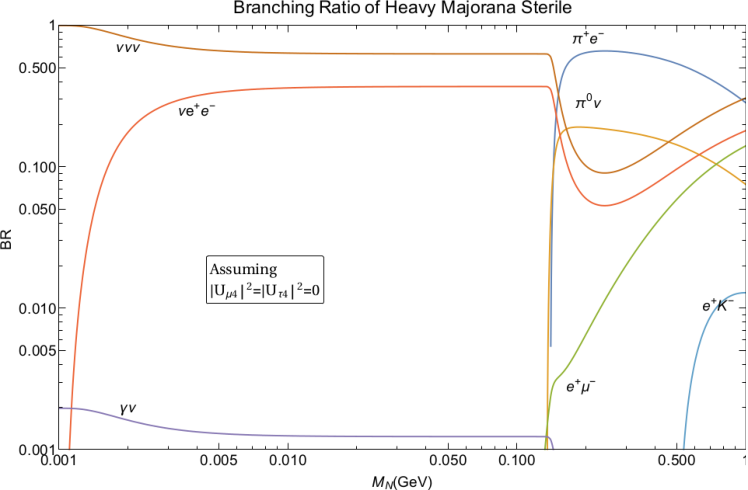
\includegraphics[width=0.49\textwidth]{figures/bounds2.pdf}
\caption{\label{fig:branchingratios}The branching ratios for sterile neutrino decays in the minimal 3 sterile SM extension. The left panel assumes equal mixing with all active flavours, whilst the right panel assumes a flavour hierarchical scheme where only the mixing with $\nu_e$ is important.}
\end{figure}

We highlight four decays in our study. These have the largest branching ratios
of all channels with visible decay products over the mass range $m_\text{s}
\lesssim 1$ GeV. This is based on the minimal sterile extension of the SM
discussed above, but we stress that similar decays can occur in any number of
non-minimal models, where the relationship between decay rate, mass and mixing
can be non-standard. For sterile neutrino masses less than the pion mass, the
dominant visible decay will be into an electron-positron pair as an be seen
from \reffig{fig:branchingratios}. The decay rate for this channel is given by 
%
\[ \Gamma\left(\nu_\text{s}\to \nu_i e^+e^-\right) =
\frac{G_\text{F}^2m_\text{s}^5}{96\pi^3}I(m_\text{s}, U^2).  \]
%
where $I(m_s)$ is an integral. \newtext{PB}{We'll have to decide how to type these things in.}
%
We will base two analyses on this channel, differentiated by the number of
tracks we expect to see. The first event sample will attempt to measure events
where two tracks are resolved, which is expected to have a small background but
favours low-energy events. The second sample studies the converse, where only a
single track can be seen, predominately due to a tightly collimated
$e^+e^-$-pair. In this case we expect a larger background (from anything
producing a single track), but as we will show, we get sizable event numbers in
this chanel due to the sterile neutrino's high energy, and a tight cut on the
angular distribution can make it sensitive to sterile decays.

When the mass of the sterile neutrino is greater than the kinematic threshold
for the production of a neutral pion, a new decay dominates
$\nu_\text{s}\to\nu_i \pi^0$. The decay rate for this process is given by
%
\[ \Gamma\left(\nu_\text{s} \to \nu_i \pi^0\right) =
\frac{G_\text{F}^2f_\pi^2m_\text{s}^3}{64\pi}\left[1-\left(\frac{m_\pi}{m_\text{s}}\right)^2\right].
\]

The next channel appears at the kinematic threshold for charged pion production
with a charged lepton. If mixing between the heavy mass state and the electron
neutrino is present, this decay occurs almost immediately after the $\nu\pi^0$
channel opens. However, if this mixing is negligible, there is a the size of
the muon mass before the $\mu^\pm\pi^\mp$ channel opens. As can be seen from
\reffig{fig:branchingratios}, these decays dominate the visible decays when
they are allowed. These decays have a similar scaling behaviour of the decay
rate to the $\nu\pi^0$ channel with an equivalent dependence on the pion
structure constant,
%
\[ \Gamma\left(\nu_\text{s} \to l^\pm\pi^\mp\right) =
\left|U_{l4}\right|^2\frac{2G_\text{F}^2f_\pi^2m_\text{s}^3}{16\pi}I(m_\text{s}).
\]


\lorem\lorem

\section{Simulation details}

We have computed the fluxes and simulated event numbers for each beam and
detector via a custom Monte Carlo program. The program allows efficiencies to
be taken into account due to experimental details of the detector and its
capabilities in a fully correlated way between observables. 

The fluxes from BNB are taken from REF, and we assume no spectral modifications
associated with the altered kinematics of the new sterile neutrino final state.
%
Given the spectral flux of sterile neutrinos in the BNB,
$\mathrm{d}\phi/\mathrm{d}E$, we compute the total number of accepted events in
channel ``$\text{c}$'' via the following summation,
%
\[ N_\text{c} = \sum_{i} \left .
\frac{\mathrm{d}\phi}{\mathrm{d}E}\right|_{E_i} P_\text{D}\left(E_i\right)
W_\text{c}\left(E_i\right),  \]
%
where $P_\text{D}(E)$ is the probability for a sterile of that energy to reach
and then decay inside the detector labelled $\text{D}$. The simplest
approximation is to ignore all geometric effects, so that every particle
travels exactly along the direction of the beam line, which gives the following
probability 
%
\[ P_\text{D}\left(E\right) = e^{-\frac{\Gamma_\text{T}L}{\gamma\beta}}\left(
1-
e^{-\frac{\Gamma_\text{T}\lambda}{\gamma\beta}}\right)\frac{\Gamma_\text{c}}{\Gamma_\text{T}},
\]
%
where $\Gamma_\text{T}$ ($\Gamma_\text{c}$) denotes the rest-frame total decay
width (decay width into channel $\text{c}$), $m$ the mass of the sterile
neutrino, and $L$ ($\lambda$) the distance to (width of) the detector. The
combination $\gamma\beta$ is the usual special relativisitic function of
velocities of the parent particle and provides the sole energy dependence of
the expression
%
\[   \frac{1}{\gamma\beta} \equiv \frac{m}{\sqrt{E^2-m^2}}. \]
%
As we are exploring a large parameter space, often this expression takes a
simplified form depending on the size of $\Gamma_\text{T}\lambda/\gamma\beta$:
%
\begin{align*} 
%
\Gamma_\text{T}\lambda \ll 1\qquad&\qquad P_\text{D} \approx
e^{-\frac{\Gamma_\text{T}L}{\gamma\beta}}\frac{\Gamma_\text{c}\lambda}{\gamma\beta}
+ \mathcal{O}\left(\Gamma_\text{T}^2\lambda^2\right),\\ 
%
\Gamma_\text{T}\lambda \gg 1\qquad&\qquad P_\text{D} \approx
e^{-\frac{\Gamma_\text{T}L}{\gamma\beta}}\frac{\Gamma_\text{c}}{\Gamma_\text{T}}
+ \mathcal{O}\left(\frac{1}{\Gamma_\text{T}\lambda}\right), 
%
\end{align*}
%
where the rate for slowly decaying particles can be seen to grow with detector
size until a width of $\lambda\sim\Gamma_\text{c}^{-1}$ where longer detectors
make no difference, as most steriles decay within a few decay lengths and
therefore we see a fixed fraction of the total events in our channel of interest. 
We will comment on how the three detectors of the SBN complex can use the 
dependence on $E$ and $L$ in these expressions to enhance their sensitivity in 
Section ??.

%
Finally, the function $W_\text{c}(E)$ is a weighting factor which accounts for
all effects which reduce the number of events in the sample: for example,
analysis cuts or detector performance effects.
%
To compute these factors, we run a Monte Carlo simulation of the decays for a
large number of sample eventsi with a given energy. Each sterile event is
associated with a decay of type $\text{c}$. We then apply experimental analysis
cuts to the decays based on our assumptions about the detector's capabilities
and backgrounds, to produce a spectrum representing the final event sample. The
percentage of accepted events defines the weight factor for that energy.

We also work spectrally producing the expected distributions of observed
events. This can be used to suggest improved analysis cuts based on the
interplay between thre three detectors of the SBN complex. We return to this in
section II.

\subsection{Sterile neutirno fluxes}

To leading order in the mass of the sterile neutrino over the pion, the fluxes
for the $\nu_\text{s}$ will be a rescaling of the fluxes for the active
neutrinos.  We take these fluxes as our input and scale them by $U_{\mu4}$, with an additional kinematic factor to take into account the helicity un-supression of $\pi^+ \rightarrow e^+\nu_s$ for massive $\nu_s \gg m_e$, such that for a sterile produced from the decay of a meson M
\[
	\phi_{\nu_s} \approx \phi_{\nu_\alpha} \vert U_{\alpha 4}\vert^2 \frac{\Gamma(M \rightarrow \nu_s \alpha)}{\Gamma(M\rightarrow \nu_\alpha \alpha)}.
\]
This kinematic effect for the pion and kaon, the only mesons produced in large numbers in the BNB beam, is shown below in figure \ref{fig:flux_enhancement}

\begin{figure}[t]
\center
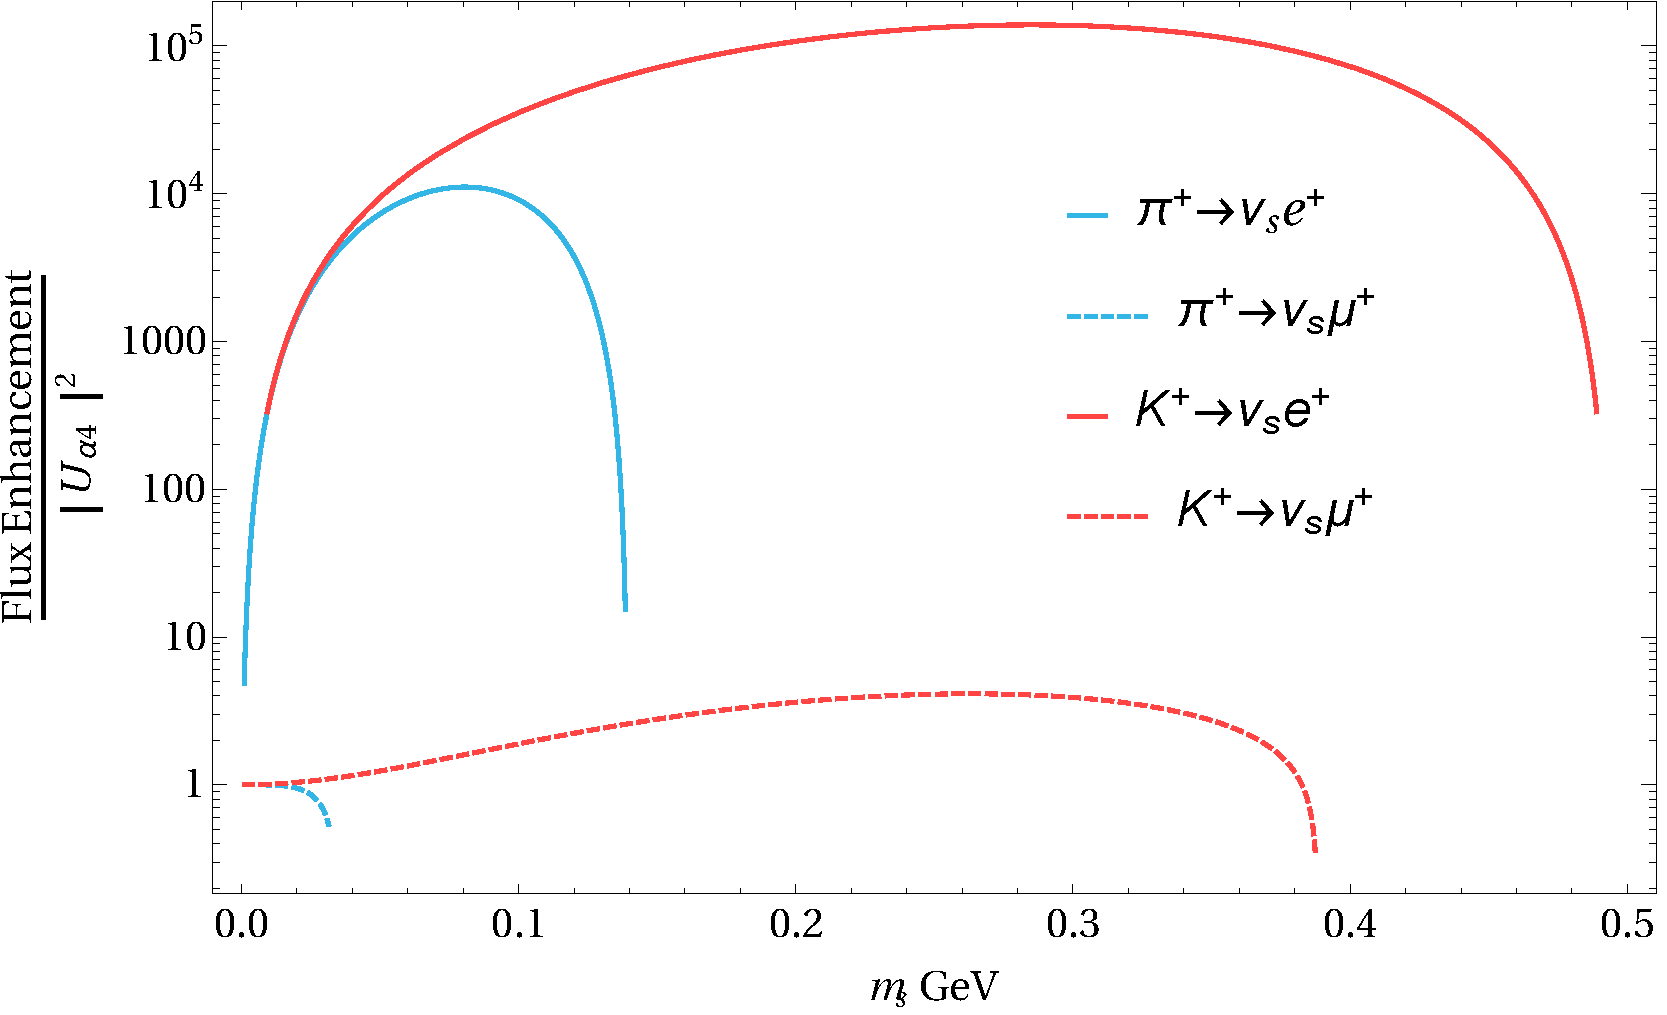
\includegraphics[width=0.6\textwidth]{figures/BNB_flux_enhancement.pdf}

\caption{\label{fig:flux_enhancement} Kinematic enhancements of the sterile flux, for the four production channels available for steriles in the BNB beam. There is little effect when mixing with muons alone, as the muon is heavy enough to remove the helicity supression that usually kills the $\pi\rightarrow e \nu$ channels. This factor of up to $10^5$ enhancement more than compensates for the smaller flux of $\nu_e$ inherent in the BNB beam.}

\end{figure}





%
\newtext{PB}{Can we add a figure of the fluxes? Perhaps some comment on how we
are modelling them. This is all finished, right? (Unless we start doing
something wild with the NuMI fluxes).}
%
\lorem\lorem 

\subsection{Detector modelling and analysis cuts}

To compute the weighting factors $W_\text{c}$, we generate a large number of
Monte Carlo events of the decay that we are interested in and remove those
events which fail a series of cuts. These cuts are designed to reflect both
genuine analysis cuts designed to enhance the signal to background ratio (for
example, choosing events with energies within certain ranges), as well as cuts
which provide a basic model of detector effects and limitations (for example,
discarding events that wouldn't be reconstructed correctly, \eg\ those with
overlapping tracks in a two particle final state).

We summarize our cuts in \reftab{tab:cuts}.
%
\begin{table}[t]
\centering
\begin{tabular}{ l | l | l}
Signal & Constraint & Value \\
\hline\hline
 \multirow{4}{*}{$e^+ e^-$ (two tracks)} & low-energy thresh. & $50$ MeV\\
 \cline{2-3}
 & foreshortened angular separation & $>5^\circ$ \\
 \cline{2-3}
 & energy ratio $E_\text{low}/E_\text{high}$ & $>0.1$\\
 \cline{2-3}
 & angle? & $100\%$\\
\cline{1-3}
 \multirow{4}{*}{$e^+ e^-$ (single track)} & low-energy thresh. & $50$ MeV\\
 \cline{2-3}
 & foreshortened angular separation & $<5^\circ$ \\
 \cline{2-3}
 & energy ratio $E_\text{low}/E_\text{high}$ & $<0.1$\\
 \cline{2-3}
 & angle? & $100\%$\\
\cline{1-3}
 \multirow{3}{*}{$\pi^+e^-(\pi^-e^+)$} & low-energy thresh. & $10$ MeV\\
 \cline{2-3}
 & energy ratio $E_e/E_\pi$ & $>0.1$\\
 \cline{2-3}
 & angle? & $100\%$\\
\cline{1-3}
 \multirow{3}{*}{$\pi^+\mu^-(\pi^-\mu^+)$} & low-energy thresh. & $10$ MeV\\
\cline{2-3}
 & energy ratio $E_\mu/E_\pi$ & $>0.1$\\
\cline{2-3}
 & angle? & $100\%$\\
\end{tabular}
\caption{\label{tab:cuts}Detector cuts as modelled in our simulation.}
\end{table}
\newpage
\newpage
\subsection{Background modelling}
For each channel, we have implemented a model of the dominant backgrounds. The
properties of these backgrounds will motivate our cuts. The knowledge of the
background and the cuts to motivate a reasonable estimate of the backgrounds to the searches of interest.  We will discuss the details of the modelling that we have performed in a channel-by-channel basis. The results of this rate only background analysis is summarised in Table (\ref{tab:Rates}) below.

\subsubsection{$\pi e$ and $\pi \mu$ channels}

Pions produced inside \muboone\ will quickly decay into muons, which
subsequently decay into Michel electrons. We can expect this chain of decays to
be well reconstructed in liquid argon, and the dominant backgrounds to the
sterile decays we are interested in will be genuine $\pi$-lepton production
associated with the neutrino beam. So-called CC1$\pi^+$ events are defined as
the associated production of a charged pion from the standard CC process which
produces a lepton. This can happen by resonant production, where a nucleon is
excited into an unstable state, for example into a $\Delta$, and the following
decay produces a nucleon and a pion. Such decays are characterised by a
isotropic spectrum due to the relatively mild boost of the resonant state
\cite{Rein:1982pf}. Another contribution to the cross-section is from coherent
scattering, where the neutrino scatters from the whole nucleus 
%
\[   \nu_l + A \to l^- + A + \pi^+ \qquad\text{or}\qquad \overline{\nu}_l + A
\to l^+ + A + \pi^-. \]
%
These interactions tend to produce more forward decay products and will be the
dominant source of our backgrounds. Cross-sections for these processes have
been studied in MiniBooNE \cite{Wascko:2006tx} and \minerva\ \cite{Eberly:2014mra} and cross-sections appear to agree with Monte Carlo
calculations based on the Rein-Sehgal model \cite{Rein:2006di, Rein:1982pf}. 

For each signal channel we consider the backgrounds which have the largest contribution. Here we focus on beam driven backgrounds, with the assumption that cosmogenic backgrounds are significantly less of an issue via timing and directional cuts. In all cases, requiring no nuclear effects should greatly reduce beam related charge current events, \newtext{MARK}{perhaps this is directly estimatable in GENIE?}.

 \begin{table}[t]
\centering
\begin{tabular}{ l | l | l}
Signal & Cut & BG Event Rate \\
\hline\hline
 \multirow{3}{*}{$e^+ e^-$ (two tracks)} & No Cuts & 3082\\
 \cline{2-3}
 & $E>200$ MeV & 1055 \\
 \cline{2-3}
 & No Vertex & 152\\
\cline{1-3}
 \multirow{4}{*}{$e^+ e^-$ (single track)} & No Cuts& 1926\\
 \cline{2-3}
 & No Hadronic Activity & 1492 \\
 \cline{2-3}
 & $E>100$ MeV  & 186 \\
 \cline{2-3}
 & \newtext{MARK}{ $1 \gamma$ BKG  } & +954?\\
\cline{1-3}
 \multirow{4}{*}{$\pi^+\mu^-(\pi^-\mu^+)$} & No Cuts & $\approx$ 40000\\
 \cline{2-3}
 & No Hadronic Activity & 5055\\
 \cline{2-3}
 & $m_\mu$ forward supression & 4034\\
 \cline{2-3}
 & Estimated Angular Cut & 2000 \\
\cline{1-3}
 \multirow{2}{*}{$\pi^+e^-(\pi^-e^+)$} & No Cuts & 310\\
\cline{2-3}
 & No Hadronic Activity  & 106\\
\cline{1-3}
\multirow{2}{*}{$\pi^0 \nu_\alpha$} & No Cuts & 9093\\
\cline{2-3}
& No Hadronic Activity  & \newtext{MARK}{1697 Coherent only}\\

\end{tabular}
\caption{\label{tab:Rates} Estimated background rates for the four channels considered in this analysis. }
\end{table}



\newtext{PB}{Can we reduce the incoherent BG by requiring no hadronic activity? What are we sensitive to? (There is usually a flying nucleon for incoherent. Unlike coherent scattering.)}

\newtext{PB}{It turns out} \cite{Rein:2006di} \newtext{PB}{that forward going events are
suppressed by muon mass. Does this mean that an angular cut could kill a lot of
our BG for $\pi \mu$? (Leaving only electron neutrino processes?)}

Additional backgrounds to the $\pi \mu$ ($\pi e$) channels will be from the
dominant backgrounds to the $\pi e$ ($\pi \mu$) channel with further particle
misidentification.

\begin{itemize}
\item {\bf $\pi^+ \mu^- (\pi^- \mu^+)$} \\
Charged coherent pion production, $\nu_\mu A \rightarrow \mu^- A \pi^+$, is large background, identical in particle content to a decaying sterile signal. Such a low $Q^2$ process tends to favour daughter pions and muons that are forward going, kinematically very similar to decays in flight, as well as no observable nuclear activity. ArgoNeut analysis estimates the approximate number of events, for similar liquid argon technology to $\mu$BooNE \cite{Acciarri:2014eit} For low energy no events have been observed thus far, see SciBooNE \cite{Tanaka:2009ag} and high energy event rates are in accordance with what is expected, see NOMAD \cite{Kullenberg:2009pu}.

There is approximately 40,000 events coherent and incoherent resonant 1$\mu$ 1 $\pi$ events produced in MicroBooNE. However, when one ensure that there is no hadronic activity this reduces to 5055, 2626 of which are CC coherent events, the remainder from incoherent events which have little or no observable hadronic activity. Any further reduction must arise from kinematic cuts. \newtext{MARK}{As you mentioned that forward going events are suppressed for our BG, if we include the 25\% suppression for coherent and 15\% for incoherent that leaves us with 4034 events. However, the real benefit here will come from out spectrum in relation the the pions. As the incoherent is relatively isotropic, the 2000 events from the coherent production will probably be our main irreducible background.} 

	
\item {\bf $\pi^+ e^- (\pi^- e^+)$} \\
	 Coherent pion production is in theory a background similar to the muon case above, however, this process has never been experimentally measured with associated electron production, and estimated event rates in microBooNE are $\mathcal{O}(10)$ events. Thus a much larger background is any traditional $\mu \pi$ production in which the muon is mis-identified as an electron, however, this should be quite small, between 50-100 events.
	\end{itemize}
	

\subsubsection{$e^+ e^-$ single and double track channels}


\begin{itemize}
\item  {\bf $e^+ e^-$ (single tracks)} \\
	Any CCQE scattering event producing a single electron acts as a possible background to sufficiently boosted $e^+e^-$ pairs. However, as this is a key background to the $\nu_e$ appearance oscillation analysis the kinematics and rates are well understood. The additional requirement that the single electron is not accompanied by any pions, as well as no nuclear proton recoils in which nuclear energy is above the threshold of 50 MeV (\newtext{MARK}{50 is probably too  large, 21 is more appropriate, however, numbers exist for 50 in easier to access papers}), reduces the background rate by approximately 30\% to 1492 events. To further improve on this one can use the resultant electron spectral shapes. As events containing no pion or protons favour forward focused electrons, mimicking a daughter electron from a sterile decay in flight, the angular spectrum does not play a significant role in background reduction. A substantial number of these electrons-like events are not true electrons but mis-id low-energy photons from $\pi^0 \rightarrow \gamma \gamma$ decay or muons, one can apply a low energy threshold cut of 100 MeV on the electron energy to reduce the number of expected events to 186 (29 with perfect proton detection). %	(see MicroBooNE Document 2149-v1).

\newtext{MARK}{Hmm, two electrons overlapping have twice the $\frac{dE}{dx}$ or a single electron, so we may have to include the single photon events as described below.}

\item {\bf $e^+ e^-$ (two tracks)} \\
The primary background to a resolvable $e^+ e^-$ two-track pair is either a single photon which pair produces two clean electrons rapidly such that the shower separation is not observable or a two photon system, such as from a NC $\pi^0 \rightarrow \gamma \gamma$ decay, in which both photons are mis-id as electrons. If one assumes that all single photon events can be a possible background to a $e^+ e^-$ search there is approximately 2088 events expected in $6.6\times10^{20}$ POT. Similarly to the single track $e^+ e^-$, most of this background is at low energies so a 200 MeV cut on photon energy reduces this significantly to 654 events. To estimate the two photon mis-identification we apply a conservative 6\% photon to electron mis-id rate to known two photon backgrounds to obtain a rate of approximately 994 events. A further cut on  energy of 200 MeV on both photons reduces this to 401. 

These can be naively combined to give 1055 (3082) with (without) a 200 MeV cut on photon energy. Additional backgrounds involving mis-id muons will not be significant in comparison to these NC pion decays and any remaining cosmic backgrounds not naturally removed by beam spill is eliminated by such a 200 MeV cut.\\

The above single photon analysis assumes the possible existence of a vertex in which to measure the photons conversion length from. In the absence of a vertex in which to measure off this can be reduced to 1389 (152) without (with) a 200 MeV energy cut. 
		
\newtext{MARK}{Effect of angular cuts? }
\end{itemize}

\subsubsection{$\pi^0 \nu_\alpha$}
Although a subdominant decay mode when steriles mix with electrons alone, when one considers non-zero $\vert U_{\mu4}\vert^2$ the branching ratio of $\nu_s \rightarrow \nu_\mu \pi^0$ becomes dominant for a mass window $\approx 140 \rightarrow 240$ MeV. Single neutral pions are produced in great numbers at the three SBN facilities, so the lack of any nuclear recoil is crucial in eliminating the majority of the incoherent neutral pion production background. The NC coherent pion production, however, does not contain any nuclear tracks and so will be an irreducible background for this channel. 

\begin{table}[t]
\centering
\begin{tabular}{ l | l }
Channel  assuming $6.6\times 10^{20}$ PoT& Num Events  \\
\hline\hline
CCQE $(\nu_\mu n \rightarrow p \mu^-)$ & 60,161 \\
NC elastic $(\nu_\mu N \rightarrow \nu_\mu N)$ & 19,409  \\
CC resonant $\pi^+$ $(\nu_\mu N \rightarrow \mu^- N \pi^+)$ & 25,149  \\
CC resonant $\pi^0$ $(\nu_\mu n \rightarrow \nu_\mu p \pi^0)$ & 6,994  \\
NC resonant $\pi^0$ $(\nu_\mu N \rightarrow \nu_\mu N \pi^0)$ & 7,388  \\
NC resonant $\pi^\pm$ $(\nu_\mu N \rightarrow \nu_\mu N^\prime \pi^\pm)$ & 4,796  \\
NC coherent $\pi^0$ $(\nu_\mu A \rightarrow \nu_\mu A \pi^0)$ & 1,694 \\
CC coherent $\pi^+$ $(\nu_\mu A \rightarrow \mu^- A \pi^+)$ & 2,626 \\
\hline
Intrinsic $\nu_e$ CC & 326 \\
CC coherent $\pi^+$ $(\nu_e A \rightarrow e^- A \pi^+,$) & 9 (my estimate) \\
\end{tabular}
\caption{\label{tab:rates}Some estimated statistics for various channels in microBooNE, as estimated using previous MiniBooNE and ArgoNeut data.}
\end{table}

\section{Sensitivities}

In \reffig{fig:no_cuts_no_bkg} we show the sensitivity when cuts are omitted
for backgroundless searches. This corresponds to the most optimistic case:
there are no cuts (weight factors are set to $1$, not even taking into account
physical limitations on the data set) implying perfect signal efficiency, and
the channels are assumed backgroundless.
%
The analysis only considers the total number of events in each channel, and the
contours mark the regions where the detectors in question see more than $2.44$
events, following the procedure of \refref{Feldman:1997qc} designed for
backgroundless searches for rare events. 

To investigate how the presence of backgrounds weaken these sensitivities, we
have performed a rough estimate of the significance of the signal in various
channels. In \reffig{fig:no_cuts_scaled_bkg}, we consider the quantity
$S/\sqrt{\lambda B}$ and plot contours when the parameter is equal to $1$. At
this point, the size of the new signal events from the heavy sterile decays are
equal to the Poisson noise in the experiment under the approximation of no
signal. The parameter $\lambda$ is used to scale the backgrounds, corresponding
to a greater ability to suppresses these events.  We show two regions, the most
conservative line corresponds to $\lambda=1$ with no additional background
suppression beyond our estimates, whilst the more optimistic one corresponds to
a further suppression by a factor of 1000. Our estimates are given by the
largest numbers in \reftab{tab:rates} for each channel, that is assuming no
analysis-based reduction in rates. As before, we do not take into account the
signal efficiency in these plots (weight factors are set to $1$) this makes the
unrealistic assumptiont that whatever has been done to reduce the backgrounds
leaves the signal event rates unchanged. However, it provides an understanding of 
the severity of the impact of the backgrounds for these searches.

\newtext{PB}{Be careful: the contours aren't really the same thing as the
shaded region, as they are computing different statistical quantities. But to
make them into actual exclusion curves, we would have to minimize over the 2D
space... which maybe we should do... but as we know it takes a bit of work.
Also, the ee flux isn't quite right for a reason I forget at the moment.}


\begin{figure}[t]
\center
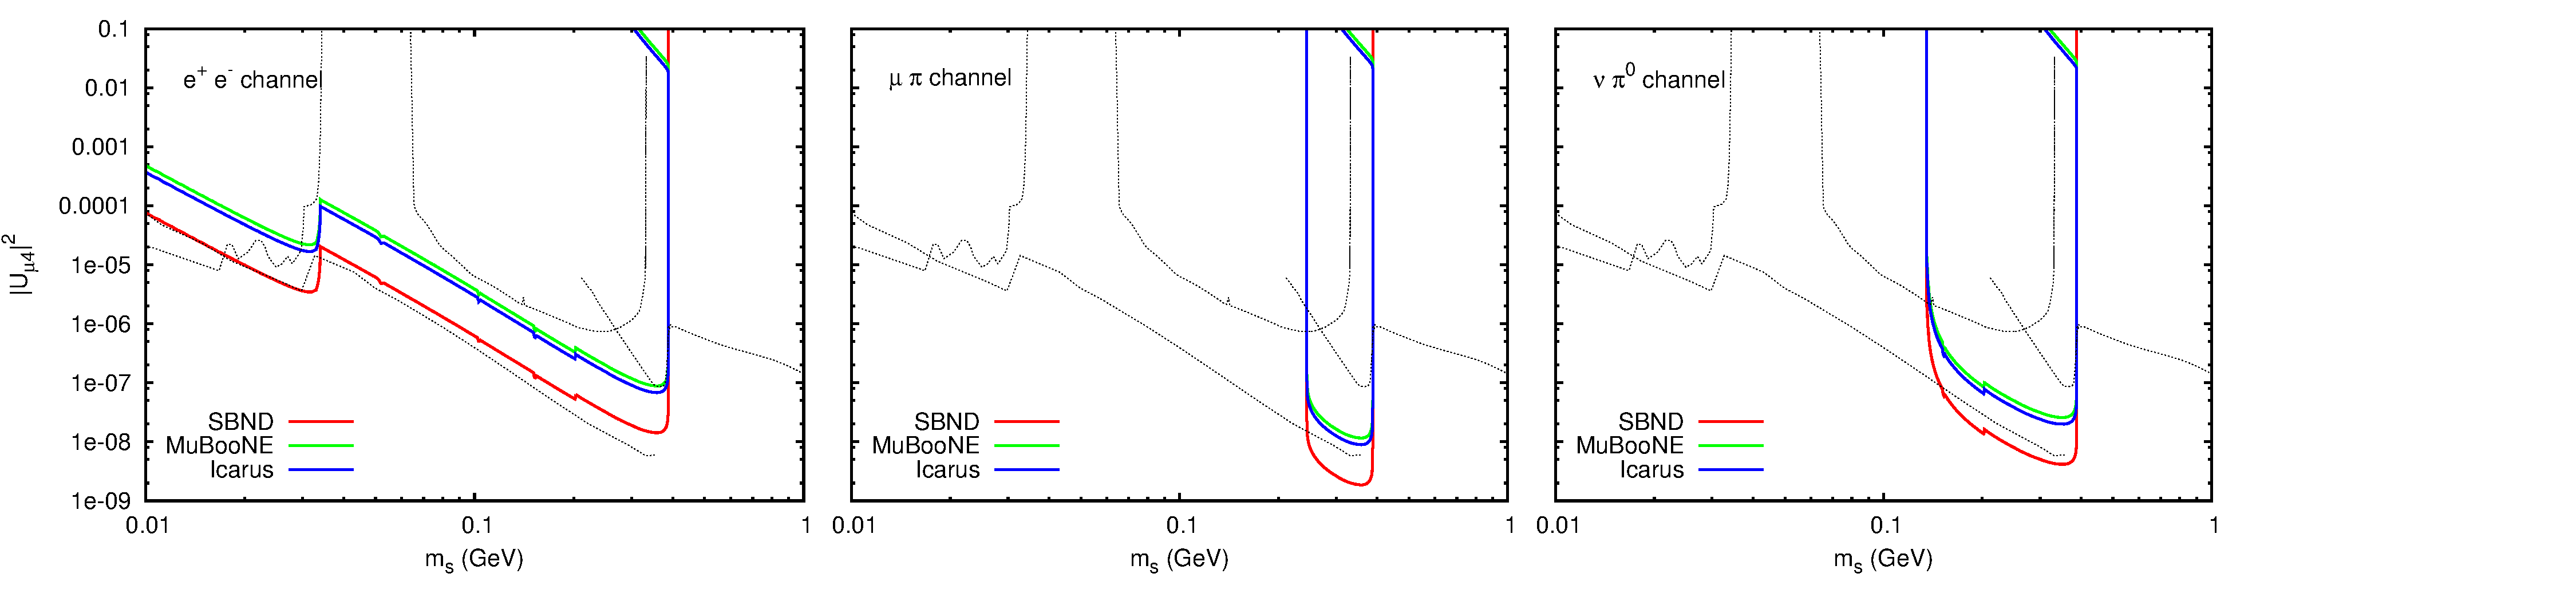
\includegraphics[width=1.0\textwidth,clip,trim=0 20 300 15]{figures/zerobg_um4_all_panels.pdf}
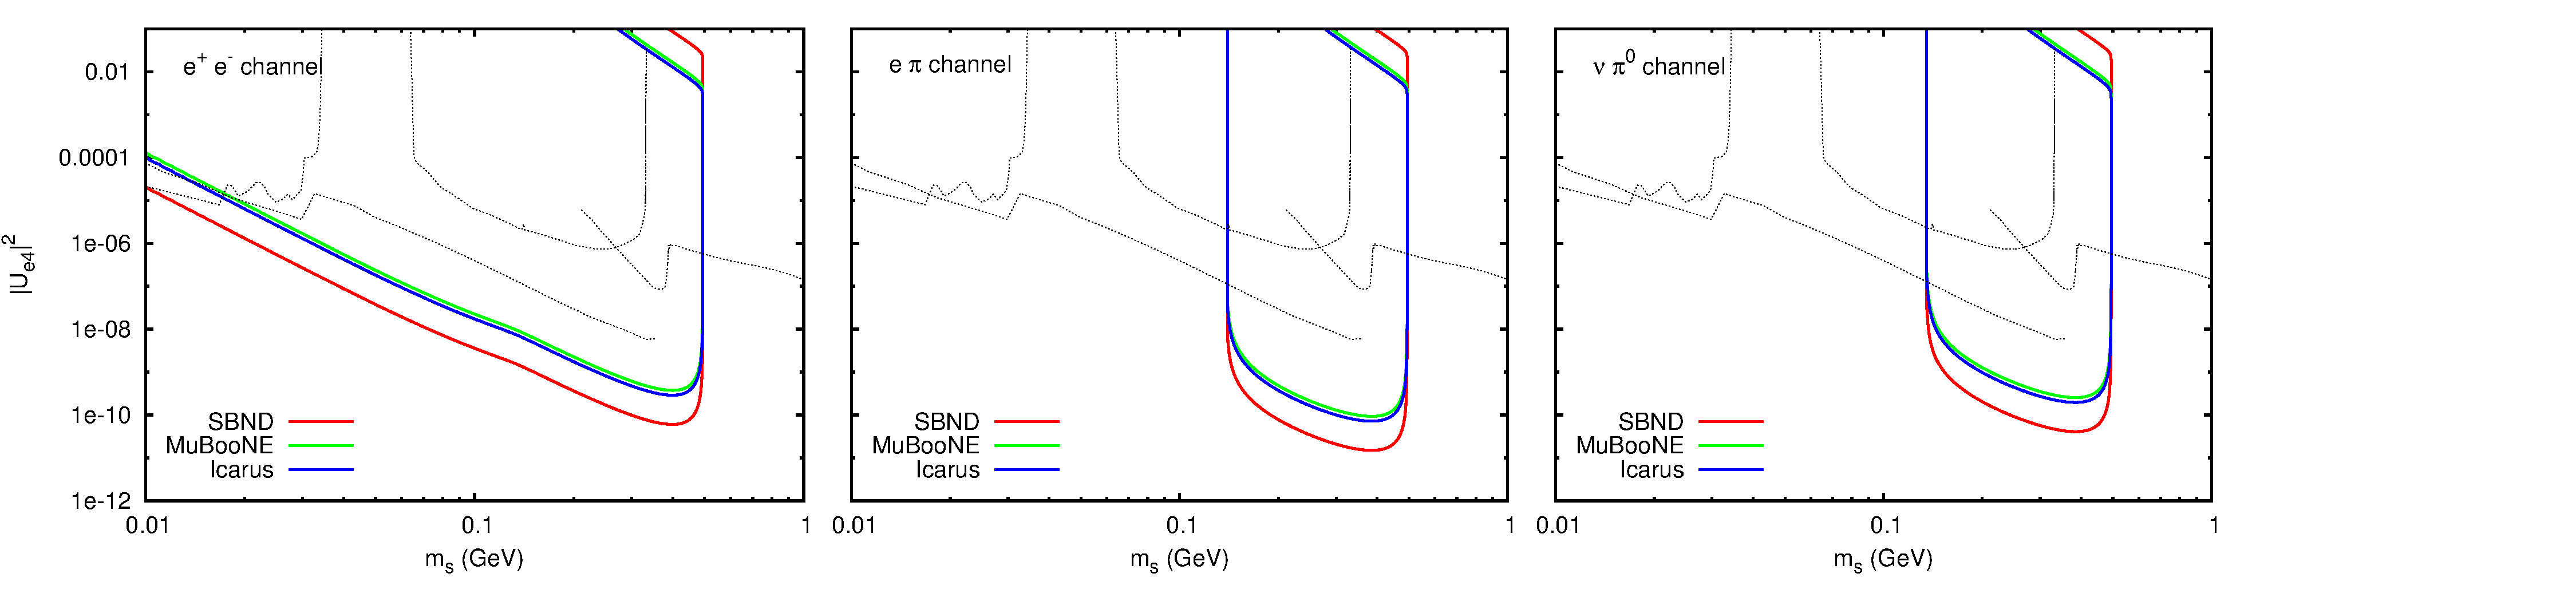
\includegraphics[width=1.0\textwidth,clip,trim=0 20 300 15]{figures/zerobg_ue4_all_panels.pdf}

\caption{\label{fig:no_cuts_no_bkg}The sensitivity contours based on the total number of events, without cuts and without backgrounds. In all panels, the mixing matrix elements not shown on the $y$-axis are zero.}

\end{figure}

\begin{figure}[t]
\center
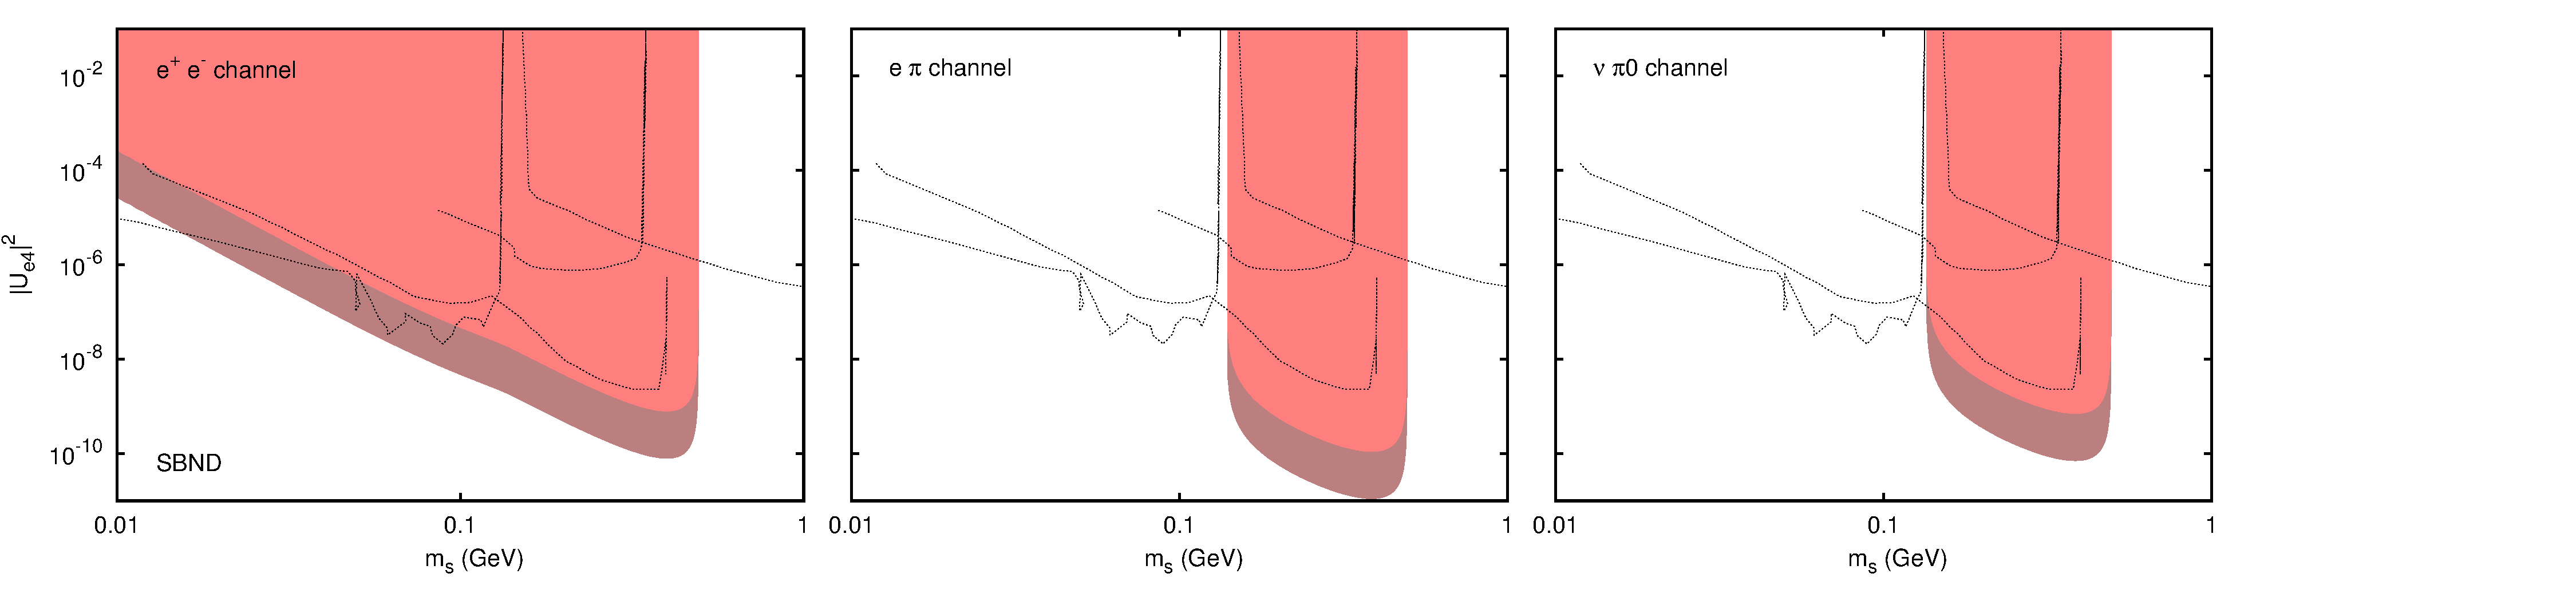
\includegraphics[width=1.0\textwidth,clip,trim=0 20 300 15]{figures/sbnd_all_panels_ue4.pdf}
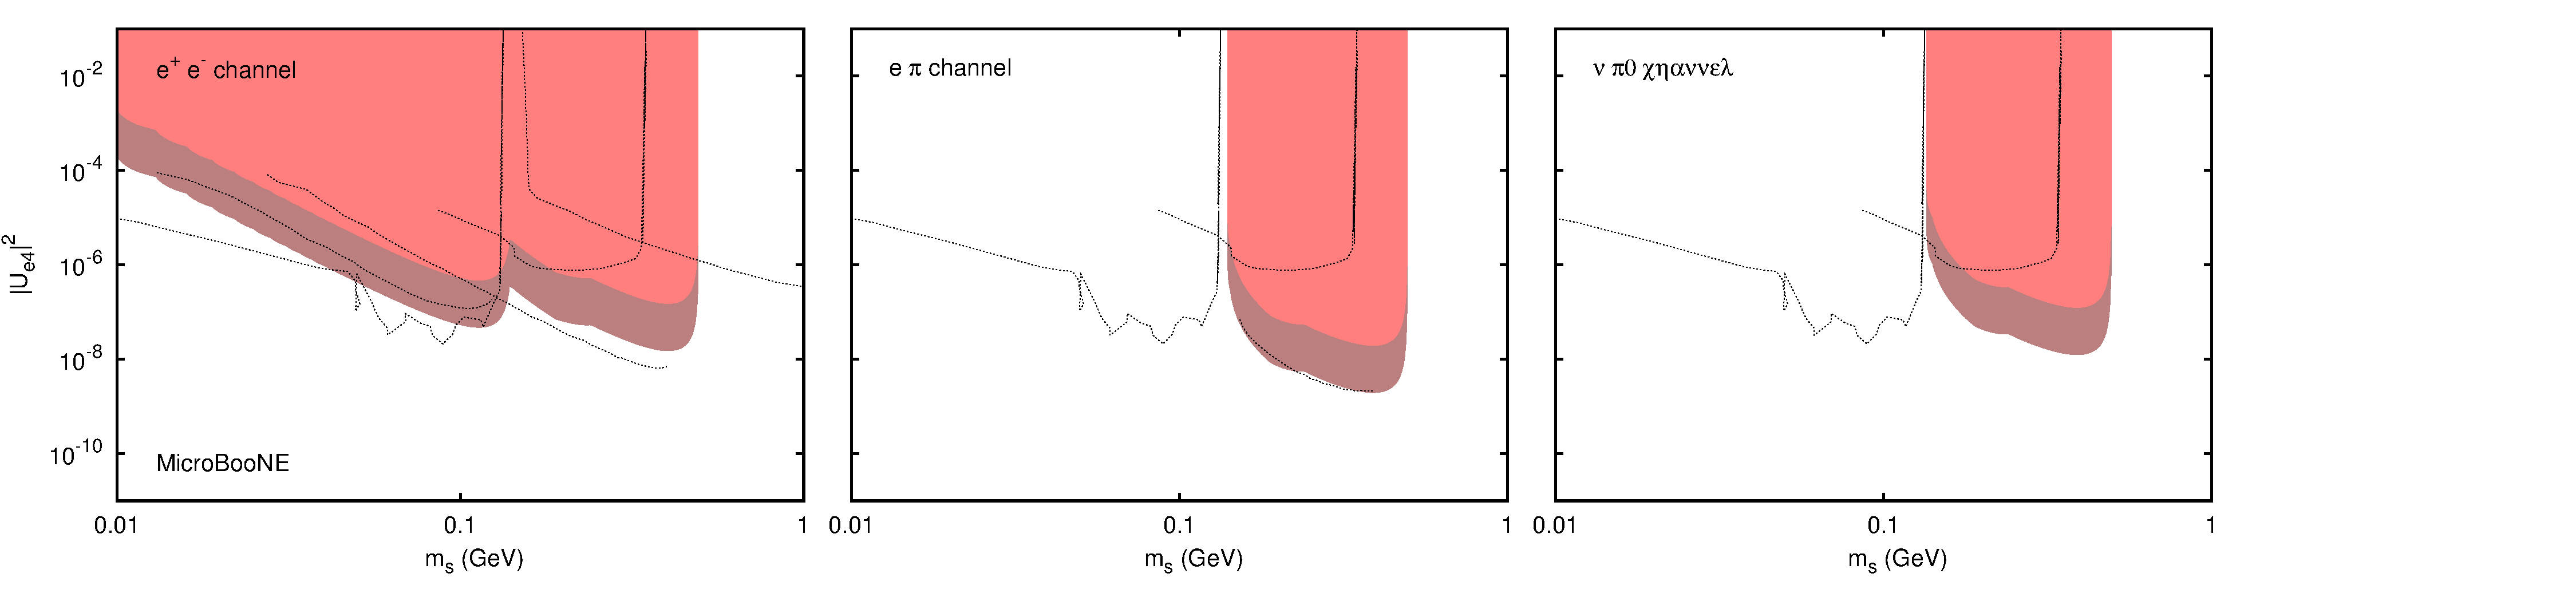
\includegraphics[width=1.0\textwidth,clip,trim=0 20 300 15]{figures/muboone_all_panels_ue4.pdf}
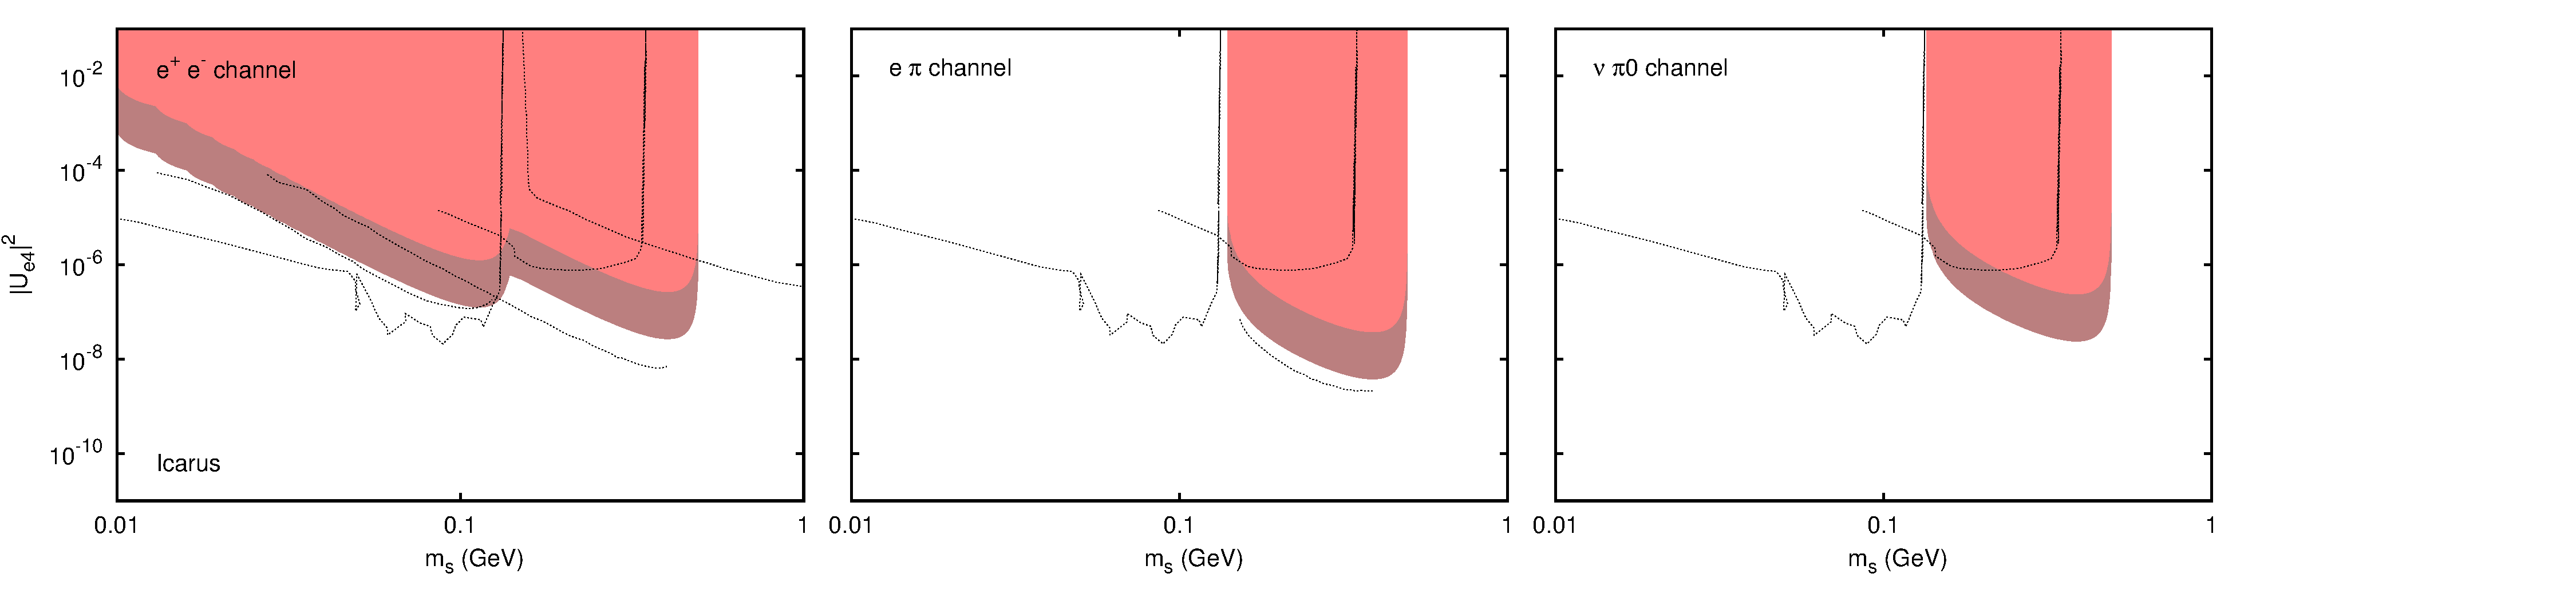
\includegraphics[width=1.0\textwidth,clip,trim=0 20 300 15]{figures/icarus_all_panels_ue4.pdf}

\caption{\label{fig:no_cuts_scaled_bkg_ue4_only}The sensitivity contours based on the total
	number of events, assuming only mixing with the electron neutrio ( $\vert U_{\mu 4}\vert^2=\vert U_{\tau 4}\vert^2=0$), without cuts but with varying degrees of background
suppression. We overlay the 95\% exclusion regions for $U^2$ and $m_s$ from
previous experimental work.}

\end{figure}

\begin{figure}[t]
\center
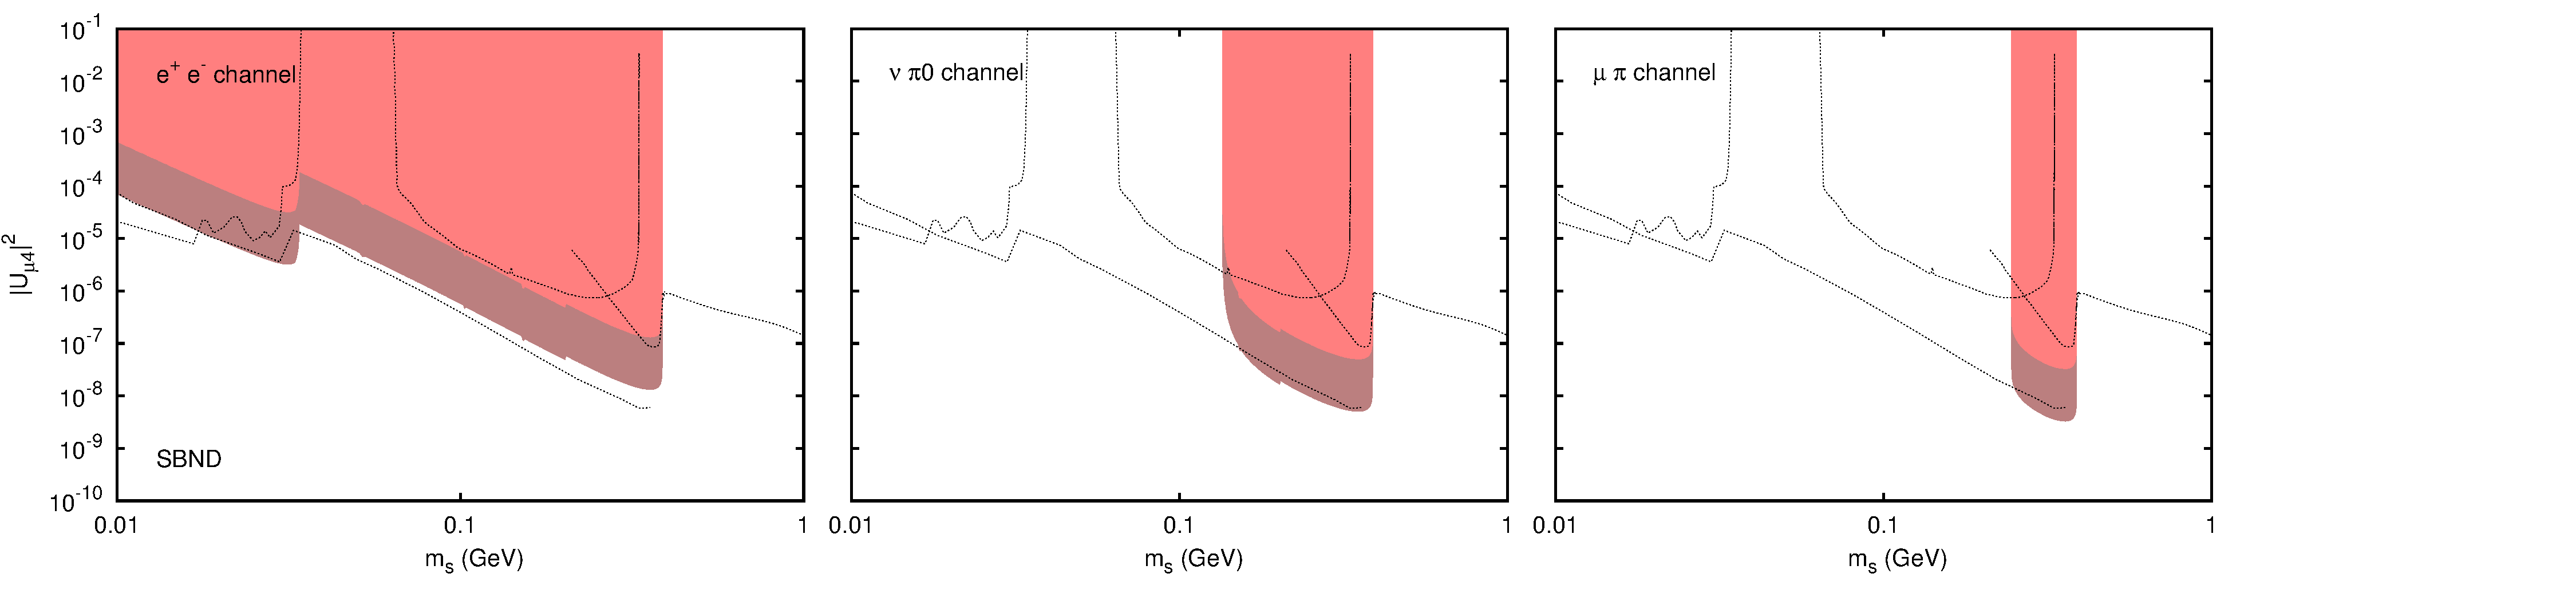
\includegraphics[width=1.0\textwidth,clip,trim=0 20 300 15]{figures/sbnd_all_panels_um4.pdf}
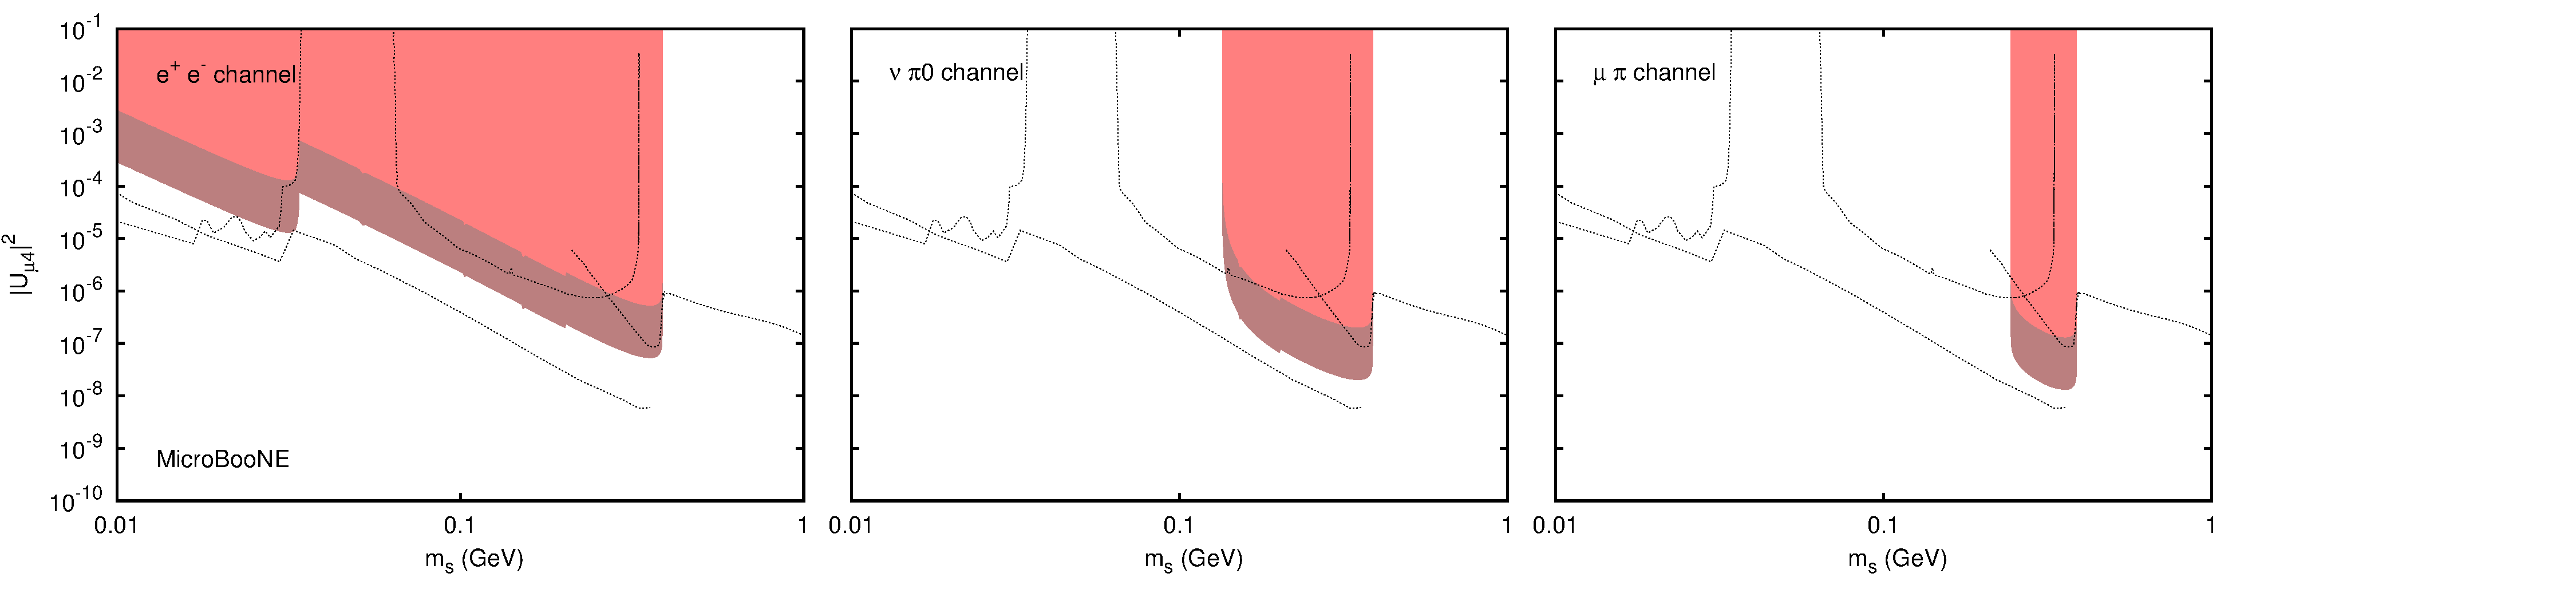
\includegraphics[width=1.0\textwidth,clip,trim=0 20 300 15]{figures/muboone_all_panels_um4.pdf}
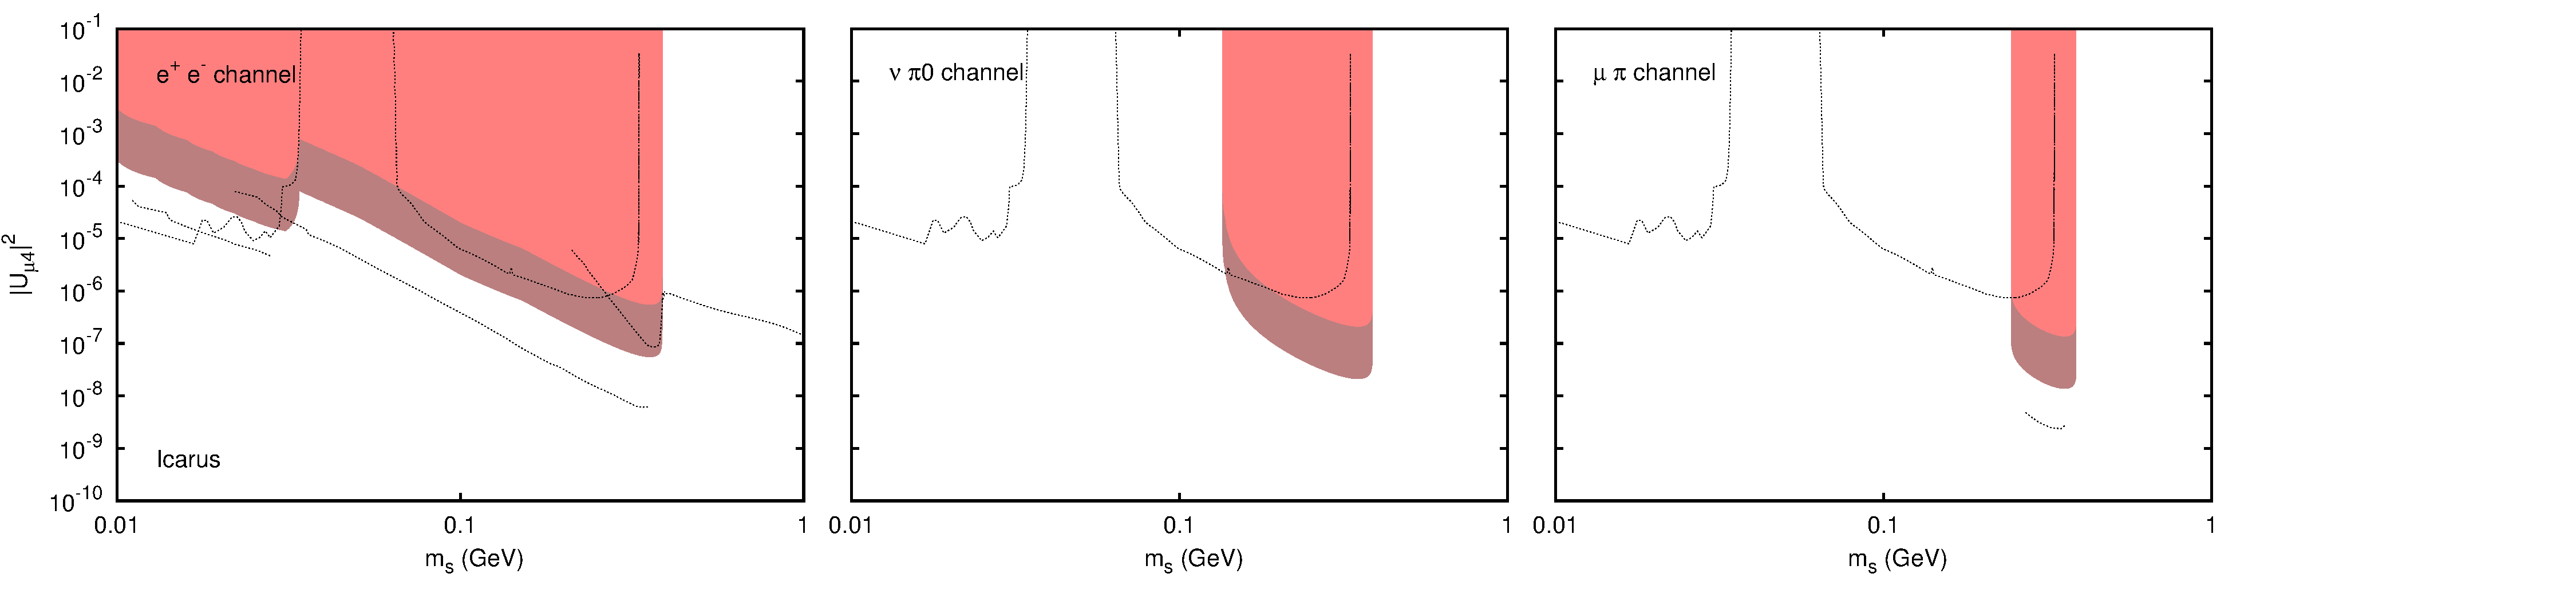
\includegraphics[width=1.0\textwidth,clip,trim=0 20 300 15]{figures/icarus_all_panels_um4.pdf}

\caption{\label{fig:no_cuts_scaled_bkg_um4_only}The sensitivity contours based on the total
number of events, assuming only mixing with the muon neutrinor ( $\vert U_{e 4}\vert^2=\vert U_{\tau 4}\vert^2=0$), without cuts but with varying degrees of background
suppression. We overlay the 95\% exclusion regions for $U^2$ and $m_s$ from
previous experimental work.}

\end{figure}


\section{Conclusions}
\lorem\lorem


\newpage 

\section{To do list}

\begin{enumerate}

%\item \sout{Add mass scaling of backgrounds to $S/\sqrt{B}$ plot.}
%\newtext{MARK}{All currently taken care of in centralised file
%"bkg\_event\_rates\_"}

%\item \sout{Work out which mixing angles are active in each plot. And overlay
%$U_{e4}$ bounds on appropriate plot. Probably: recompute plots with this
%information.}

%\item \sout{Plot for total sum of events over detectors.} \newtext{PB}{It's pointless.}

%\item \sout{Add $\nu_e$ flux to \emph{flux.c}.}

\item Actually commpute a $95\%$ CL exlusion region for a fair comparison with
bounds. \newtext{PB}{See comment directly below. (This isn't a total
solution... but I spent a while reading about how to do this properly and I
think it's pretty defensible. Perhaps more so than what we would do with
log-likelihood ratios...)}.

\item \sout{The $S/\sqrt{B} =1$ criterion is (if it's defensible at all) really a
$1\sigma$ significance measure. I think we should at least switch it to
$S/\sqrt{B} =2$ which is $2\sigma\approx 95\%$ in the Gaussian limit.}
\newtext{PB}{I have done this and updated the plotting scripts.}

\item \sout{Work out what has gone into the ``cut-less"
plots.}\newtext{PB}{``Cut-less'' plots have weight factors set to 1.} Recompute
for reasonable cuts? Vary the backgrounds according the cuts and Mark's
estimates?

%\item \sout{Play about with baseline distance? \newtext{MARK}{What can we
%really say here, if we limit to "standard" mixing picture  then there isnt a
%huge ammount of results, (see figures/baseline\_effects.pdf), might look into
%increased decay rates?} \newtext{PB}{Yes, I'm starting to think that we should
%just add a section looking at generic decay widths in specific channels... we
%have to make some decisions about how $\Gamma$ scales with $U$. I mean, just
%assuming the minimal extension \emph{is} pretty conservative for theorists.}}
%\newtext{PB}{I think we agreed to just do this.}

\item Turn on $U_{\tau 4}$,$U_{\mu 4}$ and $U_{e4}$ simultaneously

\item \sout{Edit how the code deals with cuts and efficiency files.
``--no-cuts" shouldn't need a dummy file of 1's. Maybe a flag ``--cuts-XXX``
where XXX is either a file name, or ``none'' for which all is handled
internally.} \newtext{PB}{Now there is a ``--cuts'' flag. ``--cuts=none'' or
``-cuts none'' sets all weights to 1 internally. Or you can pass it a file name
``--cuts=eff.dat'', which works as expected. Default is no cuts, but I've
updated the scripts to have the right flags.}

\item \sout{Write code for general $\Gamma$ for different final state
particles.} \newtext{PB}{I've had a first pass at this. I didn't write new
decay channels in the end, as I think we can just rescale things...  depending
on how we choose to scale the $\Gamma$ with $U$ and $m$ (see below), we could
change this later, but for now it seemed OK. Now there's a new command
line argument which adds an extra Gamma to whichever channel you specify as well 
as the total decay rate \emph{e.g.} \texttt{eventrate --mupi --extra-gamma 1e-18}
adds a constant $1\times10^{-18}$ to the $\mu\pi$ channel and total rate (not
double counting). When we write a function like \texttt{loop\_muon\_enhanced\_gamma()} we 
can set this extra gamma to depend on $U$ or $m$ as we need.} 

\item Write a section talking about the motivation for non-minimal extensions,
specifically enhanced $\Gamma$. Discuss the breaking of the relationship
between $\Gamma$, $U^2$ and $m_s$.  Make a reasonable suggestion for possible
scaling behaviours of $\Gamma$ on $U^2$/$m_s$. Is it as boring as rewriting the
minimal decay rate with $G_F$ replaced by a new constant that isn't suppressed
by the $W$-mass? Or can you get different scaling behaviours from new physics?

\item Based on the point above: decide how we can make plots for this. How do
we compute the bounds? I guess, the bounds are \emph{really} bounds on
$U^2\Gamma$? What's the best way to display the three dimensional data etc.
Make the data. Make the plots.

\end{enumerate}

%%%%%%%%%%%%%%%%%%%%%%%%%%%%%%%%
%%%%%%%%%%%%%%%%%%%%%%%%%%%%%%%%
%%%%%%%%%%%%%%%%%%%%%%%%%%%%%%%%

\bibliographystyle{apsrev4-1}
\bibliography{lib}{}

\end{document}

